%%%%%%%%%%%%%%%%%%%%%%%%%%%%%%%%%%%%%%%%%
% Beamer Presentation
% LaTeX Template
% Version 1.0 (10/11/12)
%
% This template has been downloaded from:
% http://www.LaTeXTemplates.com
%
% License:
% CC BY-NC-SA 3.0 (http://creativecommons.org/licenses/by-nc-sa/3.0/)
%
%%%%%%%%%%%%%%%%%%%%%%%%%%%%%%%%%%%%%%%%%

%----------------------------------------------------------------------------------------
%	PACKAGES AND THEMES
%----------------------------------------------------------------------------------------

% \documentclass{beamer}
\documentclass[handout]{beamer}


\mode<presentation> {

\usetheme{Madrid}

}

\definecolor{DataBlue}{rgb}{0.50, 0.85, 0.99} 

\setbeamercolor{titlelike}{parent=structure,bg=black, fg = white}
\setbeamercolor{frametitle}{fg=white}
\usepackage{graphicx} % Allows including images
\usepackage{booktabs} % Allows the use of \toprule, \midrule and \bottomrule in tables
\usepackage[export]{adjustbox}
\usepackage[portuguese]{babel}
\usepackage[utf8]{inputenc}

\usepackage{pgfplots}
\usepackage{tikz}
\usetikzlibrary{calc,babel,quotes,angles}
\usetikzlibrary{overlay-beamer-styles}
\usepackage{tkz-euclide}

\usepackage[normalem]{ulem}
\usepackage{amsmath, amsfonts, amssymb}

\usepackage{cancel}

\usepackage{multirow}
% \usepackage{xcolor}

\makeatletter
\let\save@measuring@true\measuring@true
\def\measuring@true{%
  \save@measuring@true
  \def\beamer@sortzero##1{\beamer@ifnextcharospec{\beamer@sortzeroread{##1}}{}}%
  \def\beamer@sortzeroread##1<##2>{}%
  \def\beamer@finalnospec{}%
}
\makeatother


%----------------------------------------------------------------------------------------
%	TITLE PAGE
%----------------------------------------------------------------------------------------

\title{Geometria} %% Title
\subtitle{Aula 05}
\author{Gustavo Ale} % Your name
\institute[UFMT] % Your institution as it will appear on the bottom of every slide, may be shorthand to save space
{
EduCursinho - Faculdade de Engenharia \\ % Your institution for the title page
\medskip
\textit{gustavo.engca@gmail.com} % Your email address
}
\date{19 de Setembro de 2021} % Date, can be changed to a custom date

% Rodapé
% \setbeamertemplate{footline}{%
%     \begin{beamercolorbox}[wd=\paperwidth]{footlinecolor}
%         \includegraphics[width=\paperwidth]{images/footbar.png}
%     \end{beamercolorbox}%
% }

\begin{document}
{
\setbeamertemplate{footline}{}
\begin{frame}
    \begin{columns}
        \begin{column}{0.48\textwidth}
            % \hspace*{-1cm}
            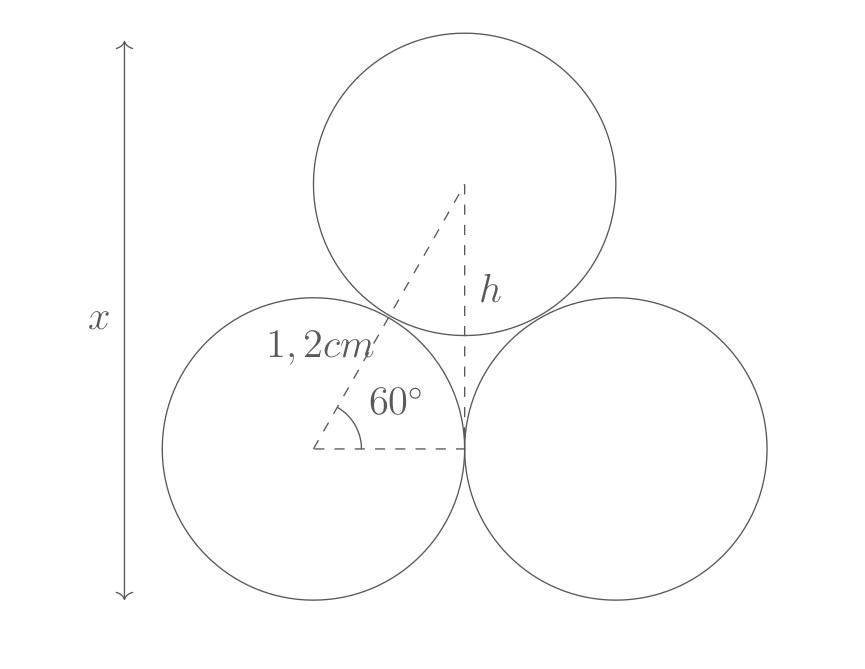
\includegraphics[width=\columnwidth,left]{../assets/geo.png}
        \end{column}
        \begin{column}{0.48\textwidth}
            \titlepage
        \end{column}
    \end{columns}

\end{frame}
}

%-------------------------------------------------------------------------------
% Sumário
%-------------------------------------------------------------------------------

\begin{frame}
    \frametitle{Sumário} % Table of contents slide, comment this block out to remove it
    \tableofcontents % Throughout your presentation, if you choose to use \section{} and \subsection{} commands, these will automatically be printed on this slide as an overview of your presentation
\end{frame}

%----------------------------------------------------------------------------------------
%	PRESENTATION SLIDES
%----------------------------------------------------------------------------------------

\section{Aulas anteriores}
\subsection{Revisão}
\begin{frame}[fragile]\frametitle{\subsecname}
    Até agora vimos como trabalhar com problemas que podem ser decompostos em um 
    ou mais triângulos retângulos, tanto através das funções trigonométricas e 
    suas relações com o triângulo retângulo, como também utilizando do Teorema 
    de Pitágoras.  
\end{frame}

%------------------------------------------------

\begin{frame}\frametitle{\subsecname}
    \begin{block}{Relações trigonométricas}
        \begin{columns}
            \begin{column}{0.2\textwidth}
                \begin{align*}
                    sen(\theta) = \frac{CO}{hip}
                \end{align*}
            \end{column} 
            \begin{column}{0.2\textwidth}
                \begin{align*}
                    cos(\theta) = \frac{CA}{hip}
                \end{align*}
            \end{column} 
            \begin{column}{0.2\textwidth}
                \begin{align*}
                    tg(\theta) = \frac{CO}{CA}
                \end{align*}
            \end{column} 

        \end{columns}
    \end{block}

    \begin{block}{Teorema de Pitágoras}
        \begin{align*}
            a^2 = b^2 + c^2
        \end{align*}
    \end{block}


\end{frame}


%------------------------------------------------

\section{Lei dos Cossenos}
% \subsection{Introdução}

\begin{frame}[fragile]\frametitle{\secname}
    Assim como o Teorema de Pitágoras, a lei dos Cossenos assemelha os comprimentos
    dos lados do triângulo, sendo possível determinar qualquer uma de suas grandezas 
    quando se sabe o comprimento de ao menos 2 lados e 1 ângulo.
    \begin{figure}[H]
        \centering
        %\resizebox{\columnwidth}{!}{%
        \begin{tikzpicture}[scale=0.8\columnwidth/10cm]
            \coordinate (A) at (0,0);
            \coordinate (B) at (5,3);
            \coordinate (C) at (7,0);

            \draw (B)-- (C)-- (A)-- (B);
            \draw (A)-- node[above left] {$a$} (B); 
            \draw (B)-- node[right] {$c$} (C); 
            \draw (C)-- node[below] {$b$} (A); 
            \pic ["$\beta$", draw, -, angle eccentricity=2] {angle = A--B--C};
            \pic ["$\alpha$", draw, -, angle eccentricity=2] {angle = B--C--A};
            \pic ["$\gamma$", draw, -, angle eccentricity=2] {angle = C--A--B};
            
        \end{tikzpicture}
        %}
        % \caption{Triângulo retângulo $ABC$}
    \end{figure}

    Enquanto o Teorema de Pitágoras funciona apenas para triângulos retângulos, 
    a Lei dos Cossenos pode ser aplicada para \textbf{qualquer triângulo}.

\end{frame}

%------------------------------------------------

\begin{frame}[fragile]\frametitle{\secname}
    \begin{figure}[H]
        \centering
        %\resizebox{\columnwidth}{!}{%
        \begin{tikzpicture}[scale=0.6\columnwidth/10cm]
            \coordinate (A) at (0,0);
            \coordinate (B) at (5,3);
            \coordinate (C) at (7,0);
            
            \draw (B)-- (C)-- (A)-- (B);
            \draw (A)-- node[above left] {$a$} (B); 
            \draw (B)-- node[right] {$c$} (C); 
            \draw (C)-- node[below] {$b$} (A); 
            \pic ["$\beta$", draw, -, angle eccentricity=2] {angle = A--B--C};
            \pic ["$\alpha$", draw, -, angle eccentricity=2] {angle = B--C--A};
            \pic ["$\gamma$", draw, -, angle eccentricity=2] {angle = C--A--B};
            
        \end{tikzpicture}
        %}
        % \caption{Triângulo retângulo $ABC$}
    \end{figure}
    % A Lei dos Cossenos é composta por 3 equações, sendo elas:
    % \begin{align*}
    %     a^2 = b^2 + c^2 - 2\cdot b\cdot c\cdot cos(\alpha)\\
    %     b^2 = a^2 + c^2 - 2\cdot a\cdot c\cdot cos(\beta)\\ 
    %     c^2 = a^2 + b^2 - 2\cdot a\cdot b\cdot cos(\gamma)   
    % \end{align*}
    \begin{block}{A Lei dos Cossenos é composta por 3 equações, sendo elas:}
        \begin{align*}
            a^2 = b^2 + c^2 - 2\cdot b\cdot c\cdot cos(\alpha)\\
            b^2 = a^2 + c^2 - 2\cdot a\cdot c\cdot cos(\beta)\\ 
            c^2 = a^2 + b^2 - 2\cdot a\cdot b\cdot cos(\gamma)   
        \end{align*}
    \end{block}
    
\end{frame}

%------------------------------------------------

\begin{frame}\frametitle{\secname}
    \Huge{\centerline{Mas como decorar essa \sout{joça?}}}
\end{frame}

%------------------------------------------------
\begin{frame}[fragile]\frametitle{\secname}
    \begin{figure}[H]
        \centering
        %\resizebox{\columnwidth}{!}{%
        \begin{tikzpicture}[scale=0.6\columnwidth/10cm]
            \coordinate (A) at (0,0);
            \coordinate (B) at (5,3);
            \coordinate (C) at (7,0);
            
            \draw (B)-- (C)-- (A)-- (B);
            \draw[color=red!50] (A)-- node[above left] {$a$} (B); 
            \draw (B)-- node[right] {$c$} (C); 
            \draw (C)-- node[below] {$b$} (A); 
            \pic ["$\beta$", draw, -, angle eccentricity=2] {angle = A--B--C};
            \pic ["$\alpha$", draw, -, angle eccentricity=2] {angle = B--C--A};
            \pic ["$\gamma$", draw, -, angle eccentricity=2] {angle = C--A--B};
            % \draw[color=red,visible on=<2->] (B) -- node[above left] {$a$} (A); 
            \draw[color=blue!50,visible on=<2->] (C) -- node[below] {$b$} (A); 
            \draw[color=blue!50,visible on=<2->] (C) -- node[right] {$c$} (B); 
            \pic [color=orange,"$\alpha$", draw, -, angle eccentricity=2, visible on=<3->] {angle = B--C--A};
        \end{tikzpicture}
        %}
        % \caption{Triângulo retângulo $ABC$}
    \end{figure}
    Supondo que queremos o comprimento \textcolor{red!50}{$a$}, \onslide<2-> então começamos com $a^2$ sendo igual a
    soma do quadrado das demais medidas. \onslide<3-> Depois subtraimos por 2 vezes
    o produto das demais medidas e o cosseno do ângulo oposto à aresta \textcolor{red!50}{$a$}, no caso 
    o ângulo \textcolor{orange}{$\alpha$}
    \begin{align*}
        \onslide<2-> \textcolor{red!50}{a^2} &= \textcolor{blue!50}{b^2 + c^2} \onslide<3-> 
        - 2\cdot \textcolor{blue!50}{b\cdot c\cdot} cos(\textcolor{orange}{\alpha})
    \end{align*}
    \begin{alertblock}{}
        Isso serve para qualquer um dos lados.
    \end{alertblock}

    
\end{frame}

%------------------------------------------------

\begin{frame}%\frametitle{\secname}
    \begin{block}{Lei dos Cossenos}
        \begin{align*}
            a^2 = b^2 + c^2 - 2\cdot b\cdot c\cdot cos(\alpha)\\
            b^2 = a^2 + c^2 - 2\cdot a\cdot c\cdot cos(\beta)\\ 
            c^2 = a^2 + b^2 - 2\cdot a\cdot b\cdot cos(\gamma)   
        \end{align*}
    \end{block}
\end{frame}

%------------------------------------------------

\section{Exemplos}
\begin{frame}[fragile]\frametitle{\secname}
    \begin{block}{Exemplo 1.}
        Dado o triângulo abaixo, calcule o comprimento de $x$:
        \begin{figure}[H]
            \centering
            %\resizebox{\columnwidth}{!}{%
            \begin{tikzpicture}[scale=0.5\columnwidth/10cm]
                \coordinate (A) at (0,0);
                \coordinate (B) at (4,4);
                \coordinate (C) at (5,0);
                
                \draw (B)-- (C)-- (A)-- (B);
                \draw (A)-- node[above left] {$4cm$} (B); 
                \draw (B)-- node[above right] {$3cm$} (C); 
                \draw (C)-- node[below] {$x$} (A); 
                \pic ["$60^\circ$", draw, -, angle eccentricity=1.5] {angle = A--B--C};
                % \pic ["$\alpha$", draw, -, angle eccentricity=1.5] {angle = B--C--A};
                % \pic ["$\gamma$", draw, -, angle eccentricity=1.5] {angle = C--A--B};

            \end{tikzpicture}
            %}
            % \caption{Triângulo retângulo $ABC$}
        \end{figure}
    \end{block}

\end{frame}
%------------------------------------------------

\begin{frame}[fragile]\frametitle{\secname}
    \begin{columns}
        \begin{column}{0.5\columnwidth}
            \begin{figure}[H]
                % \centering
                %\resizebox{\columnwidth}{!}{%
                \begin{tikzpicture}[scale=1\columnwidth/10cm]
                    \coordinate (A) at (0,0);
                    \coordinate (B) at (4,4);
                    \coordinate (C) at (5,0);
                    
                    \draw (B)-- (C)-- (A)-- (B);
                    \draw (A)-- node[above left] {$4cm$} (B); 
                    \draw (B)-- node[above right] {$3cm$} (C); 
                    \draw (C)-- node[below] {$x$} (A); 
                    \pic ["$60^\circ$", draw, -, angle eccentricity=1.5] {angle = A--B--C};
                    % \pic ["$\alpha$", draw, -, angle eccentricity=1.5] {angle = B--C--A};
                    % \pic ["$\gamma$", draw, -, angle eccentricity=1.5] {angle = C--A--B};
                    
                \end{tikzpicture}
                %}
                % \caption{Triângulo retângulo $ABC$}
            \end{figure}
        \end{column}

        \begin{column}{0.5\textwidth}
            Vamos começar por escrever a equação que rege esse problema.
            \begin{align*}
                x^2 &= 3^2 + 4^2 \pause- 2\cdot3\cdot4\pause\cdot \cos{(60^\circ)}\\
                \pause x^2 &= 25 - 24\cos{(60^\circ)}\\
                \pause x^2 &= 25 - \frac{24}{2} = 25-12 = 13\\
                \pause x &= \sqrt{13} \approx  \boxed{3,60}
            \end{align*}
        \end{column}
    \end{columns}

\end{frame}

%------------------------------------------------

\section{Exemplos}
\begin{frame}[fragile]\frametitle{\secname}
    Podemos também encontrar o valor de um ângulo dado as dimensões do triângulo.
    \begin{block}{Exemplo 2.}
        Dado o triângulo abaixo, calcule o ângulo $\alpha$:
        \begin{figure}[H]
            \centering
            %\resizebox{\columnwidth}{!}{%
            \begin{tikzpicture}[scale=0.5\columnwidth/10cm]
                \coordinate (A) at (1,0);
                \coordinate (B) at (-1,4);
                \coordinate (C) at (7,0);
                
                \draw (B)-- (C)-- (A)-- (B);
                \draw (A)-- node[left] {$3cm$} (B); 
                \draw (B)-- node[above right] {$7cm$} (C); 
                \draw (C)-- node[below] {$5cm$} (A); 
                \pic ["$\alpha$", draw, -, angle eccentricity=1.5] {angle = C--A--B};
                % \pic ["$\alpha$", draw, -, angle eccentricity=1.5] {angle = B--C--A};
                % \pic ["$\gamma$", draw, -, angle eccentricity=1.5] {angle = C--A--B};

            \end{tikzpicture}
            %}
            % \caption{Triângulo retângulo $ABC$}
        \end{figure}
    \end{block}

\end{frame}

%------------------------------------------------

\begin{frame}[fragile]\frametitle{\secname}

    \begin{columns}
        \begin{column}{0.5\columnwidth}
            
            \begin{figure}[H]
                \centering
                \begin{tikzpicture}[scale=1\columnwidth/10cm]
                    \coordinate (A) at (1,0);
                    \coordinate (B) at (-1,4);
                    \coordinate (C) at (7,0);
                    
                    \draw (B)-- (C)-- (A)-- (B);
                    \draw (A)-- node[left] {$3cm$} (B); 
                    \draw (B)-- node[above right] {$7cm$} (C); 
                    \draw (C)-- node[below] {$5cm$} (A); 
                    \pic ["$\alpha$", draw, -, angle eccentricity=1.5] {angle = C--A--B};
                    % \pic ["$\alpha$", draw, -, angle eccentricity=1.5] {angle = B--C--A};
                    % \pic ["$\gamma$", draw, -, angle eccentricity=1.5] {angle = C--A--B};
                    
                \end{tikzpicture}
            \end{figure}
        \end{column}
        
        \begin{column}{0.5\columnwidth} 
            \begin{align*}
                \pause 7^2 &= 5^2 + 3^2 \pause - 2\cdot5\cdot3\pause\cdot \cos{(\alpha)}\\
                \pause 49 &= 25 + 9 - 30\cdot \cos{(\alpha)}\\
                \pause 49-34&=-30\cdot \cos{(\alpha)}\\
                \pause 15 &= -30\cdot \cos{(\alpha)}\\
                \pause -\frac{15}{30} &= \cos{(\alpha)}\\
                \pause \cos{(\alpha)} &= -\frac{1}{2}\\
                \pause \alpha &= 120^\circ
            \end{align*}
        \end{column}
        
    \end{columns}


\end{frame}

%------------------------------------------------

%------------------------------------------------


% \section{Triângulos retângulos}
% \subsection{Teorema de Pitágoras}
% \begin{frame}[fragile]\frametitle{\secname}
% O Teorema de Pitágoras é uma nova identidade presente nas dimensões do triângulo 
% retângulo. Ela nos diz que:\\
% \begin{alertblock}{}
%     \textit{o quadrado do comprimento da hipotenusa é igual a soma dos 
%     quadrados dos comprimentos dos catetos.}\\
% \end{alertblock}
% \begin{block}{Traduzindo para uma forma matemática temos então:}
%     \begin{align*}
%         a^2 &= b^2 + c^2
%     \end{align*}
%     Onde $a$ é o comprimento da hipotenusa, $b$ e $c$ o comprimento dos catetos.
% \end{block}
% \end{frame}
% %------------------------------------------------

% \begin{frame}[fragile]\frametitle{\secname}
%     Dado o triângulo retângulo abaixo:
%     \begin{figure}[H]
%         \centering
%         %\resizebox{\columnwidth}{!}{%
%         \begin{tikzpicture}[scale=0.5\columnwidth/10cm]
%             \coordinate (A) at (0,0);
%             \coordinate (B) at (4,3);
%             \coordinate (C) at (4,0);

%             \tkzMarkRightAngle[size=.3](A,C,B);
%             \draw (B)-- (C)-- (A)-- (B);
%             \draw (A)-- node[above left] {$a$} (B); 
%             \draw (B)-- node[right] {$c$} (C); 
%             \draw (C)-- node[below] {$b$} (A); 
%             % \draw (A)-- node[above left] {$4$} (B);
%         \end{tikzpicture}
%         %}
%         % \caption{Triângulo retângulo $ABC$}
%     \end{figure}
%     O teorema nos diz que é possível obter o comprimento de 
%     qualquer um dos lados, mesmo que os ângulos internos sejam desconhecidos, sendo 
%     apenas necessário saber ao menos dois comprimentos desse triângulo.
% \end{frame}

% %------------------------------------------------

% \begin{frame}[fragile]\frametitle{\secname}
%     Em outras palavras, o teorema nos diz que a área em \textcolor{cyan}{ciano} é igual a soma das
%     áreas \textcolor{blue!50}{azul} e \textcolor{red!50}{vermelho}.
%     \begin{figure}[H]
%         \centering
%         %\resizebox{\columnwidth}{!}{%
%         \begin{tikzpicture}[scale=0.5\columnwidth/10cm]
%             \coordinate (A) at (0,0);
%             \coordinate (B) at (4,3);
%             \coordinate (C) at (4,0);
%             \coordinate (D) at (7,3);
%             \coordinate (E) at (7,0);
%             \coordinate (F) at (0,-4);
%             \coordinate (G) at (4,-4);
%             \coordinate (H) at (-3,4);
%             \coordinate (I) at (1,7);
%             \draw[dashed, fill=blue!25] (B)--(D)--(E)--(C);
%             \draw[dashed, fill=red!25] (A)--(F)--(G)--(C);
%             \draw[dashed, fill=cyan!25] (A)--(H)--(I)--(B);

%             \tkzMarkRightAngle[size=.3](A,C,B);
%             \draw (B)-- (C)-- (A)-- (B);
%             \draw (A)-- node[above left] {$a$} (B); 
%             \draw (B)-- node[right] {$c$} (C); 
%             \draw (C)-- node[below] {$b$} (A); 
%             % \draw (A)-- node[above left] {$4$} (B);
%         \end{tikzpicture}
%         %}
%         % \caption{Triângulo retângulo $ABC$}
%     \end{figure}
% \end{frame}
% %------------------------------------------------

% \subsection{Aplicações}
% \begin{frame}[fragile]\frametitle{\secname}
%     Um uso muito comum para o Teorema de Pitágoras é o cálculo da distância 
%     entre dois pontos em um plano cartesiano.
%     \begin{figure}[H]
%         \centering
%         \begin{tikzpicture}[scale=0.7\columnwidth/10cm]
%             \begin{axis}[ymin=0,ymax=5,xmin=0,xmax=5]
%                 \addplot[mark=*] coordinates {(1,1)} node[above] {$(1,1)$};
%                 \addplot[mark=*] coordinates {(4,3)} node[above] {$(4,3)$};
%                 \draw(axis cs:1,1) -- node[above] {$a$} (axis cs:4,3);
%                 \draw[dashed] (axis cs:1,1) -- node[below] {$b$} (axis cs:4,1);
%                 \draw[dashed] (axis cs:4,1) -- node[right] {$c$} (axis cs:4,3);
%             \end{axis}
%         \end{tikzpicture}
%     \end{figure}
% \end{frame}

% %------------------------------------------------

% \begin{frame}[fragile]\frametitle{\secname}
%     De modo geral, dado um ponto $P = (x_1,y_1)$ e um ponto $Q = (x_2,y_2)$ o 
%     cateto $b$ tem comprimento $|x_2-x_1|$ e o cateto $c$ tem comprimento $|y_2-y_1|$
%     \begin{figure}[H]
%         \centering
%         %\resizebox{\columnwidth}{!}{%
%         \begin{tikzpicture}[scale=0.5\columnwidth/10cm]
%             \coordinate (A) at (0,0);
%             \coordinate (B) at (5,2);
%             \coordinate (C) at (5,0);
%             % \coordinate (D) at (0,3);
%             \node[circle, fill, label={above:$(x_1,y_1)$}, inner sep=1.5pt] at (A) {};
%             \node[circle, fill, label={above:$(x_2,y_2)$}, inner sep=1.5pt] at (B) {};
%             % \node[circle, fill, label={left:$D$}, inner sep=2pt] at (D) {};
%             % \draw[dashed] (A)--(D)--(B);
%             \draw (A)-- node[above] {$a$} (B);
%             \draw[dashed] (C)-- node[below] {$b$} (A);
%             \draw[dashed] (B)-- node[right] {$c$} (C);
%         \end{tikzpicture}
%         %}
%         % \caption{Triângulo retângulo $ABC$}
%     \end{figure}
%     Utilizando do teorema de Pitágoras onde $a^2 = b^2 + c^2$ temos que:
%     \begin{align*}
%         a^2 &= |x_2-x_1|^2 + |y_2-y_1|^2\\[1ex]
%         a &= \sqrt{|x_2-x_1|^2 + |y_2-y_1|^2}
%     \end{align*}
% \end{frame}

% %------------------------------------------------

% \begin{frame}[fragile]\frametitle{\secname}

%     \begin{block}{Distância entre pontos}
%     Portanto a distância entre dois pontos quaisquer em um plano cartesiano 
%     pode ser obtida através da fórmula:
%     \begin{align*}
%         a &= \sqrt{|x_2-x_1|^2 + |y_2-y_1|^2}
%     \end{align*}
%     \end{block}
% \end{frame}


%------------------------------------------------


%------------------------------------------------


\begin{frame}
    \Huge{\centerline{Perguntas?}}
\end{frame}

%----------------------------------------------------------------------------------------

\end{document}